% !TEX program = xelatex
\documentclass[a4paper,11pt]{article}

% ============================================================
% PACKAGES
% ============================================================
\usepackage[a4paper, top=0mm, bottom=0mm, left=0mm, right=0mm]{geometry}
\usepackage{fontspec}
\usepackage[table]{xcolor}
\usepackage{tikz}
\usepackage{tabularx}
\usepackage{booktabs}
\usepackage{enumitem}
\usepackage{fancyhdr}
\usepackage{tcolorbox}
\usepackage{parskip}
\usepackage{multicol}
\usepackage{graphicx}
\usepackage{hyperref}
\usepackage{amssymb}
\usepackage{pifont}
\usepackage{setspace}

\tcbuselibrary{skins,breakable}

% ============================================================
% COLORS
% ============================================================
\definecolor{navy}{HTML}{1A2744}
\definecolor{darknavy}{HTML}{0F1B33}
\definecolor{gold}{HTML}{C8A45C}
\definecolor{goldlight}{HTML}{FDF6E3}
\definecolor{textdark}{HTML}{111827}
\definecolor{textbody}{HTML}{374151}
\definecolor{textmuted}{HTML}{6B7280}
\definecolor{textlight}{HTML}{9CA3AF}
\definecolor{grayline}{HTML}{E5E7EB}
\definecolor{graybg}{HTML}{F3F4F6}
\definecolor{greenstatus}{HTML}{059669}
\definecolor{reddanger}{HTML}{DC2626}
\definecolor{redpale}{HTML}{FEF2F2}
\definecolor{redtext}{HTML}{991B1B}
\definecolor{bluepale}{HTML}{EFF6FF}
\definecolor{bluetext}{HTML}{1E40AF}

% ============================================================
% FONTS — Lato (Premium modern sans-serif)
% ============================================================
\setmainfont{Lato}[
  UprightFont    = Lato-Regular,
  BoldFont       = Lato-Bold,
  ItalicFont     = Lato-Italic,
  BoldItalicFont = Lato-BoldItalic,
]
\newfontfamily\latoheavy{Lato Heavy}[BoldFont = Lato-Heavy]
\newfontfamily\latolight{Lato Light}[UprightFont = Lato-Light, ItalicFont = Lato-LightItalic]
\newfontfamily\latosemibold{Lato Semibold}[UprightFont = Lato-Semibold]
\newfontfamily\latoblack{Lato Black}[UprightFont = Lato-Black]
\newfontfamily\latothin{Lato Thin}[UprightFont = Lato-Thin]
\newfontfamily\latomedium{Lato Medium}[UprightFont = Lato-Medium]

\hypersetup{hidelinks}

% ============================================================
% PAGE STYLE
% ============================================================
\pagestyle{fancy}
\fancyhf{}
\renewcommand{\headrulewidth}{0pt}
\renewcommand{\footrulewidth}{0pt}

% ============================================================
% CUSTOM COMMANDS
% ============================================================
\newcommand{\sectionnum}[1]{%
  \tikz[baseline=(char.base)]{
    \node[fill=navy, text=white, circle, inner sep=0pt, minimum size=20pt, font=\latosemibold\fontsize{9pt}{9pt}\selectfont] (char) {#1};
  }%
}

\newcommand{\pageheader}[1]{%
  \noindent
  \begin{tikzpicture}[remember picture, overlay]
    \draw[grayline, line width=0.8pt] ([yshift=-2pt]current page.north west) ++(25mm,-20mm) -- ++(165mm,0);
  \end{tikzpicture}
  \begin{minipage}[t]{0.5\textwidth}
    {\fontsize{11pt}{11pt}\selectfont{\latosemibold\color{navy}SGBS Group} {\latolight\color{gold}Pty Ltd}}
  \end{minipage}%
  \hfill
  \begin{minipage}[t]{0.48\textwidth}
    \raggedleft{\fontsize{7pt}{7pt}\selectfont\latolight\color{textlight}SGBS/PD/2026-001\;\textbullet\;Property Denvour\;\textbullet\;February 2026}
  \end{minipage}
  \vspace{14pt}
}

\newcommand{\pagefooter}[1]{%
  \vfill
  \noindent\textcolor{grayline}{\rule{\textwidth}{0.4pt}}\\[4pt]
  {\fontsize{7pt}{7pt}\selectfont\latolight\color{textlight}SGBS Group Pty Ltd\;\textbullet\;Inspiring Dreams\hfill Page #1 of 7}
}

% ============================================================
\begin{document}
\thispagestyle{empty}

% ============================================================
% PAGE 1 — COVER PAGE
% ============================================================

\begin{tikzpicture}[remember picture, overlay]
  % Full page dark background
  \fill[darknavy] (current page.north west) rectangle (current page.south east);
  
  % Subtle gradient overlay
  \fill[navy, opacity=0.35] (current page.north west) rectangle ([yshift=0.45\paperheight]current page.south east);
  
  % Gold accent strip on right edge
  \fill[gold] ([xshift=-3.5pt]current page.north east) rectangle ([xshift=0pt]current page.south east);

  % Subtle geometric accents
  \draw[white, opacity=0.03, line width=0.5pt] ([xshift=-40mm, yshift=-30mm]current page.north east) circle (80mm);
  \draw[white, opacity=0.02, line width=0.5pt] ([xshift=-40mm, yshift=-30mm]current page.north east) circle (95mm);

  % === TOP BAR ===
  \draw[white, opacity=0.06, line width=0.4pt] ([yshift=-52mm]current page.north west) ++(25mm,0) -- ++(170mm,0);
  
  % Logo
  \node[anchor=north west, text=white] at ([xshift=25mm, yshift=-18mm]current page.north west) {
    {\latoheavy\fontsize{15pt}{15pt}\selectfont SGBS GROUP}\;{\latolight\fontsize{15pt}{15pt}\selectfont\color{gold}PTY LTD}
  };
  \node[anchor=north west, text=white, opacity=0.30] at ([xshift=25mm, yshift=-29mm]current page.north west) {
    {\latolight\fontsize{7pt}{7pt}\selectfont\addfontfeature{LetterSpace=14}CONSULTING \& ADVISORY SERVICES}
  };
  
  % Reference top right
  \node[anchor=north east, text=white, opacity=0.35] at ([xshift=-18mm, yshift=-18mm]current page.north east) {
    {\latolight\fontsize{8pt}{12pt}\selectfont
    \begin{tabular}{@{}r@{}}
      Proposal Ref: SGBS/PD/2026-001\\
      Date: 18 February 2026
    \end{tabular}}
  };
  
  % === MAIN TITLE AREA ===
  \fill[gold] ([xshift=25mm, yshift=-88mm]current page.north west) rectangle ++(50pt, 2pt);
  
  \node[anchor=north west, text=gold] at ([xshift=25mm, yshift=-97mm]current page.north west) {
    {\latosemibold\fontsize{9pt}{9pt}\selectfont\addfontfeature{LetterSpace=12}INSPIRING DREAMS}
  };
  
  \node[anchor=north west, text=white] at ([xshift=25mm, yshift=-114mm]current page.north west) {
    {\latoblack\fontsize{42pt}{50pt}\selectfont
    \begin{tabular}{@{}l@{}}
      Year-End\\
      Accounting\\
      Services
    \end{tabular}}
  };
  
  \node[anchor=north west, text=white, opacity=0.50, text width=135mm] at ([xshift=25mm, yshift=-190mm]current page.north west) {
    {\latolight\fontsize{11.5pt}{17pt}\selectfont
    A comprehensive engagement covering financial year-end closure,
    deposit reclassification, refund reconciliation, account management,
    and the preparation of annual financial statements.}
  };
  
  % === BOTTOM STRIP ===
  \draw[white, opacity=0.06, line width=0.4pt] ([yshift=55mm]current page.south west) ++(25mm,0) -- ++(170mm,0);
  
  \node[anchor=south west, text=gold] at ([xshift=25mm, yshift=40mm]current page.south west) {
    {\latosemibold\fontsize{7pt}{7pt}\selectfont\addfontfeature{LetterSpace=8}PREPARED FOR}
  };
  \node[anchor=south west, text=white, opacity=0.65] at ([xshift=25mm, yshift=22mm]current page.south west) {
    {\latolight\fontsize{9.5pt}{14pt}\selectfont
    \begin{tabular}{@{}l@{}}
      David\\
      {\latosemibold Property Denvour}
    \end{tabular}}
  };
  
  \node[anchor=south east, text=gold] at ([xshift=-18mm, yshift=40mm]current page.south east) {
    {\latosemibold\fontsize{7pt}{7pt}\selectfont\addfontfeature{LetterSpace=8}PREPARED BY}
  };
  \node[anchor=south east, text=white, opacity=0.65] at ([xshift=-18mm, yshift=22mm]current page.south east) {
    {\latolight\fontsize{9.5pt}{14pt}\selectfont
    \begin{tabular}{@{}r@{}}
      Sibusiso Mavuso\\
      {\latosemibold SGBS Group Pty Ltd}
    \end{tabular}}
  };
\end{tikzpicture}

\clearpage

% ============================================================
% PAGE 2 — PURPOSE, BACKGROUND, ABOUT
% ============================================================
\newgeometry{top=20mm, bottom=20mm, left=25mm, right=25mm}
\thispagestyle{empty}

\pageheader{2}

{\fontsize{15pt}{15pt}\selectfont\latosemibold\color{navy}\sectionnum{1}\;\;Purpose of This Proposal}

\vspace{8pt}
{\color{textbody}\fontsize{10.5pt}{16pt}\selectfont
This proposal is submitted by \textbf{SGBS Group Pty Ltd} to Property Denvour in response to your request for assistance with the financial year-end closure and related accounting corrections.

The purpose of this document is to:}

\vspace{6pt}
\begin{tcolorbox}[colback=bluepale, colframe=bluepale, boxrule=0pt, left=4mm, right=4mm, top=3mm, bottom=3mm, borderline west={3pt}{0pt}{bluetext!80}]
{\color{bluetext}\fontsize{9.5pt}{16pt}\selectfont
\textbf{1.}\;Set out our understanding of the work required\\
\textbf{2.}\;Define the scope, deliverables, and timeline\\
\textbf{3.}\;Present the value this engagement will deliver\\
\textbf{4.}\;Provide a transparent, fixed-fee investment for your consideration}
\end{tcolorbox}

\vspace{14pt}
{\fontsize{15pt}{15pt}\selectfont\latosemibold\color{navy}\sectionnum{2}\;\;Background}

\vspace{8pt}
{\color{textbody}\fontsize{10.5pt}{16pt}\selectfont
Property Denvour manages a residential property portfolio comprising \textbf{16 occupied units}. Over the course of the current financial year, certain accounting entries require correction to ensure the books accurately reflect the financial position of the entity.

Specifically, tenant deposits have been recorded as \textbf{revenue}, whereas they are refundable amounts that should be classified as \textbf{liabilities}. Additionally, deposit refunds paid via the bank have not been allocated against the relevant tenant accounts, and several former tenants remain active in the system despite having vacated.

These matters must be resolved before the financial year can be closed and reliable financial statements produced.}

\vspace{6pt}
\begin{tcolorbox}[colback=goldlight, colframe=goldlight, boxrule=0pt, left=4mm, right=4mm, top=3mm, bottom=3mm, borderline west={3pt}{0pt}{gold}]
{\color{textbody}\fontsize{9.5pt}{14pt}\selectfont\textbf{Our commitment:} SGBS Group Pty Ltd will ensure a clean, compliant, and tax-efficient year-end --- giving you full confidence in your financial position.}
\end{tcolorbox}

\vspace{14pt}
{\fontsize{15pt}{15pt}\selectfont\latosemibold\color{navy}\sectionnum{3}\;\;About SGBS Group Pty Ltd}

\vspace{8pt}
{\color{textbody}\fontsize{10.5pt}{16pt}\selectfont
SGBS Group Pty Ltd is a consulting and advisory firm providing accounting, financial management, and business advisory services to businesses across South Africa. We combine technical accounting expertise with practical, hands-on execution --- delivering outcomes, not just paperwork.

Our approach is value-driven. We partner with clients to ensure their financial records are accurate, compliant, and decision-ready. Every engagement is designed to create clarity and confidence in the numbers.}

\pagefooter{2}

\clearpage

% ============================================================
% PAGE 3 — UNDERSTANDING YOUR NEEDS
% ============================================================
\thispagestyle{empty}

\pageheader{3}

{\fontsize{15pt}{15pt}\selectfont\latosemibold\color{navy}\sectionnum{4}\;\;Understanding Your Needs}

\vspace{8pt}
{\color{textbody}\fontsize{10.5pt}{16pt}\selectfont
Based on your instructions, the following matters require attention:}

\vspace{10pt}
{\fontsize{11pt}{11pt}\selectfont\latosemibold\color{navy}\hspace{2pt}\textcolor{gold}{\rule{2.5pt}{11pt}}\hspace{8pt}4.1\;\;Deposits Incorrectly Classified as Revenue}

\vspace{6pt}
{\color{textbody}\fontsize{10.5pt}{16pt}\selectfont
Tenant deposits received during the financial year have been recorded against a \textbf{revenue account}. Per accounting standards, refundable deposits constitute a \textbf{liability} --- not income. These must be reclassified from Revenue to a Balance Sheet liability account (e.g., ``Tenant Deposits Held'').}

\vspace{4pt}
\begin{tcolorbox}[colback=redpale, colframe=redpale, boxrule=0pt, left=4mm, right=4mm, top=3mm, bottom=3mm, borderline west={3pt}{0pt}{reddanger}]
{\color{redtext}\fontsize{9pt}{14pt}\selectfont\textbf{$\triangle$ Risk if not corrected:} Revenue is overstated, liabilities are understated, and the entity may be paying income tax on amounts that do not constitute taxable income.}
\end{tcolorbox}

\vspace{10pt}
{\fontsize{11pt}{11pt}\selectfont\latosemibold\color{navy}\hspace{2pt}\textcolor{gold}{\rule{2.5pt}{11pt}}\hspace{8pt}4.2\;\;Unallocated Deposit Refunds}

\vspace{6pt}
{\color{textbody}\fontsize{10.5pt}{16pt}\selectfont
Deposit refunds have been processed through the bank account but remain \textbf{unallocated} in the accounting records. These transactions must be identified from bank data, matched to the correct tenant, and applied against the corresponding deposit payable to reduce the liability.}

\vspace{4pt}
\begin{tcolorbox}[colback=goldlight, colframe=goldlight, boxrule=0pt, left=4mm, right=4mm, top=3mm, bottom=3mm, borderline west={3pt}{0pt}{gold}]
{\color{textbody}\fontsize{9pt}{14pt}\selectfont\textbf{\checkmark\;Outcome:} Each tenant's deposit account will accurately reflect the net liability --- deposits received less refunds paid.}
\end{tcolorbox}

\vspace{10pt}
{\fontsize{11pt}{11pt}\selectfont\latosemibold\color{navy}\hspace{2pt}\textcolor{gold}{\rule{2.5pt}{11pt}}\hspace{8pt}4.3\;\;Inactive Account Cleanup}

\vspace{6pt}
{\color{textbody}\fontsize{10.5pt}{16pt}\selectfont
Former tenants who have vacated and received their deposit refunds should be marked \textbf{inactive} in QuickBooks. Only the 16 current occupants should remain as active accounts. Accounts with open balances will be flagged and discussed with you individually before any changes are made.}

\vspace{10pt}
{\fontsize{11pt}{11pt}\selectfont\latosemibold\color{navy}\hspace{2pt}\textcolor{gold}{\rule{2.5pt}{11pt}}\hspace{8pt}4.4\;\;Year-End Closure \& Financial Statements}

\vspace{6pt}
{\color{textbody}\fontsize{10.5pt}{16pt}\selectfont
Upon completion of all corrections and adjustments, the financial year will be formally closed and a full set of \textbf{financial statements} prepared --- including an Income Statement, Balance Sheet, and supporting schedules.}

\pagefooter{3}

\clearpage

% ============================================================
% PAGE 4 — ACTIVE TENANT REGISTER + VALUE
% ============================================================
\thispagestyle{empty}

\pageheader{4}

{\fontsize{14pt}{14pt}\selectfont\latosemibold\color{navy}\sectionnum{5}\;\;Active Tenant Register}

\vspace{3pt}
{\color{textbody}\fontsize{9.5pt}{13pt}\selectfont
The following tenant accounts will remain \textbf{active}. All other accounts will be deactivated following review.}

\vspace{6pt}

\begingroup
\renewcommand{\arraystretch}{1.12}
\fontsize{8.5pt}{11pt}\selectfont
\arrayrulecolor{grayline}
\begin{tabularx}{\textwidth}{p{20mm} X p{18mm}}
\toprule
\rowcolor{navy}
{\color{white}\latosemibold\footnotesize UNIT} &
{\color{white}\latosemibold\footnotesize TENANT NAME} &
{\color{white}\latosemibold\footnotesize STATUS} \\
\midrule
Unit 1 & Refilwe Mogoshane & {\color{greenstatus}\latosemibold Active} \\
\rowcolor{graybg}
Unit 2 & Thato Raphefo & {\color{greenstatus}\latosemibold Active} \\
Unit 3 \& 4 & Siphiwe Mabusela & {\color{greenstatus}\latosemibold Active} \\
\rowcolor{graybg}
Unit 5 & Puleng Tleane & {\color{greenstatus}\latosemibold Active} \\
Unit 6 & John Moganetsi & {\color{greenstatus}\latosemibold Active} \\
\rowcolor{graybg}
Unit 7 & Sydney Nkogatsi & {\color{greenstatus}\latosemibold Active} \\
Unit 8 & Tumelo Banda & {\color{greenstatus}\latosemibold Active} \\
\rowcolor{graybg}
Unit 9 & Anele Yanda & {\color{greenstatus}\latosemibold Active} \\
Unit 10 & Mponabe Mangope & {\color{greenstatus}\latosemibold Active} \\
\rowcolor{graybg}
Unit 11 & Paballo Nkwe & {\color{greenstatus}\latosemibold Active} \\
Unit 12 & Oarabile Tlhapi & {\color{greenstatus}\latosemibold Active} \\
\rowcolor{graybg}
Unit 13 & Tshegofatso Moche & {\color{greenstatus}\latosemibold Active} \\
Unit 14 & Katlego Thlasi & {\color{greenstatus}\latosemibold Active} \\
\rowcolor{graybg}
Unit 15 & Archie Rabothata & {\color{greenstatus}\latosemibold Active} \\
Unit 16 & Tsholofelo Makatsane & {\color{greenstatus}\latosemibold Active} \\
\bottomrule
\end{tabularx}
\endgroup

\vspace{8pt}
{\fontsize{14pt}{14pt}\selectfont\latosemibold\color{navy}\sectionnum{6}\;\;The Value We Deliver}

\vspace{4pt}
\begin{minipage}[t]{0.48\textwidth}
\begin{tcolorbox}[colback=white, colframe=grayline, boxrule=0.5pt, arc=3pt, left=3mm, right=3mm, top=2.5mm, bottom=2.5mm, borderline north={2pt}{0pt}{gold}]
{\color{gold}\fontsize{9pt}{9pt}\selectfont$\blacklozenge$}\;{\color{navy}\latosemibold\fontsize{9pt}{9pt}\selectfont Accurate Financial Statements}\\[1pt]
{\color{textmuted}\fontsize{8pt}{11pt}\selectfont Deposits correctly reflected as liabilities, revenue showing only earned income, and a true financial position.}
\end{tcolorbox}
\vspace{4pt}
\begin{tcolorbox}[colback=white, colframe=grayline, boxrule=0.5pt, arc=3pt, left=3mm, right=3mm, top=2.5mm, bottom=2.5mm, borderline north={2pt}{0pt}{gold}]
{\color{gold}\fontsize{9pt}{9pt}\selectfont$\blacklozenge$}\;{\color{navy}\latosemibold\fontsize{9pt}{9pt}\selectfont Tax-Ready Position}\\[1pt]
{\color{textmuted}\fontsize{8pt}{11pt}\selectfont Correctly classifying deposits as liabilities avoids paying income tax on non-revenue amounts.}
\end{tcolorbox}
\end{minipage}%
\hfill
\begin{minipage}[t]{0.48\textwidth}
\begin{tcolorbox}[colback=white, colframe=grayline, boxrule=0.5pt, arc=3pt, left=3mm, right=3mm, top=2.5mm, bottom=2.5mm, borderline north={2pt}{0pt}{gold}]
{\color{gold}\fontsize{9pt}{9pt}\selectfont$\blacklozenge$}\;{\color{navy}\latosemibold\fontsize{9pt}{9pt}\selectfont Tenant Deposit Schedule}\\[1pt]
{\color{textmuted}\fontsize{8pt}{11pt}\selectfont A clear reconciliation per tenant --- deposits received, refunds made, and net liability outstanding.}
\end{tcolorbox}
\vspace{4pt}
\begin{tcolorbox}[colback=white, colframe=grayline, boxrule=0.5pt, arc=3pt, left=3mm, right=3mm, top=2.5mm, bottom=2.5mm, borderline north={2pt}{0pt}{gold}]
{\color{gold}\fontsize{9pt}{9pt}\selectfont$\blacklozenge$}\;{\color{navy}\latosemibold\fontsize{9pt}{9pt}\selectfont Clean Working Environment}\\[1pt]
{\color{textmuted}\fontsize{8pt}{11pt}\selectfont Only active tenants visible in QuickBooks. No clutter, fewer errors, and ready for the new year.}
\end{tcolorbox}
\end{minipage}

\pagefooter{4}

\clearpage

% ============================================================
% PAGE 5 — SCOPE OF WORK + TIMELINE
% ============================================================
\thispagestyle{empty}

\pageheader{5}

{\fontsize{15pt}{15pt}\selectfont\latosemibold\color{navy}\sectionnum{7}\;\;Scope of Work}

\vspace{6pt}
{\color{textbody}\fontsize{10.5pt}{16pt}\selectfont
The engagement is structured in five distinct phases:}

\vspace{10pt}

\begingroup
\renewcommand{\arraystretch}{1.5}
\fontsize{9.5pt}{13pt}\selectfont
\arrayrulecolor{grayline}
\begin{tabularx}{\textwidth}{>{\centering\arraybackslash}p{14mm} p{28mm} X}
\toprule
\rowcolor{navy}
{\color{white}\latosemibold\footnotesize PHASE} &
{\color{white}\latosemibold\footnotesize DELIVERABLE} &
{\color{white}\latosemibold\footnotesize DESCRIPTION} \\
\midrule
{\tikz\node[fill=navy, text=white, rounded corners=2pt, inner sep=3pt, font=\latosemibold\tiny]{1};} & {\latosemibold Deposit Reclass} & {\color{textbody}Create/verify the liability account. Identify all deposits recorded as revenue. Process reclassification journals.} \\
\rowcolor{graybg}
{\tikz\node[fill=navy, text=white, rounded corners=2pt, inner sep=3pt, font=\latosemibold\tiny]{2};} & {\latosemibold Refund Allocation} & {\color{textbody}Review bank transactions. Identify all deposit refunds. Allocate to correct tenant payables. Reconcile balances.} \\
{\tikz\node[fill=navy, text=white, rounded corners=2pt, inner sep=3pt, font=\latosemibold\tiny]{3};} & {\latosemibold Deposit Schedule} & {\color{textbody}Prepare tenant-by-tenant deposit reconciliation: received, refunded, and net outstanding at year-end.} \\
\rowcolor{graybg}
{\tikz\node[fill=navy, text=white, rounded corners=2pt, inner sep=3pt, font=\latosemibold\tiny]{4};} & {\latosemibold Account Cleanup} & {\color{textbody}Deactivate non-active accounts. Flag accounts with open balances. Confirm active 16 accounts.} \\
{\tikz\node[fill=navy, text=white, rounded corners=2pt, inner sep=3pt, font=\latosemibold\tiny]{5};} & {\latosemibold Year-End \& AFS} & {\color{textbody}Final adjustments. Close financial period. Prepare Income Statement, Balance Sheet, and schedules.} \\
\bottomrule
\end{tabularx}
\endgroup

\vspace{20pt}
{\fontsize{15pt}{15pt}\selectfont\latosemibold\color{navy}\sectionnum{8}\;\;Timeline}

\vspace{14pt}
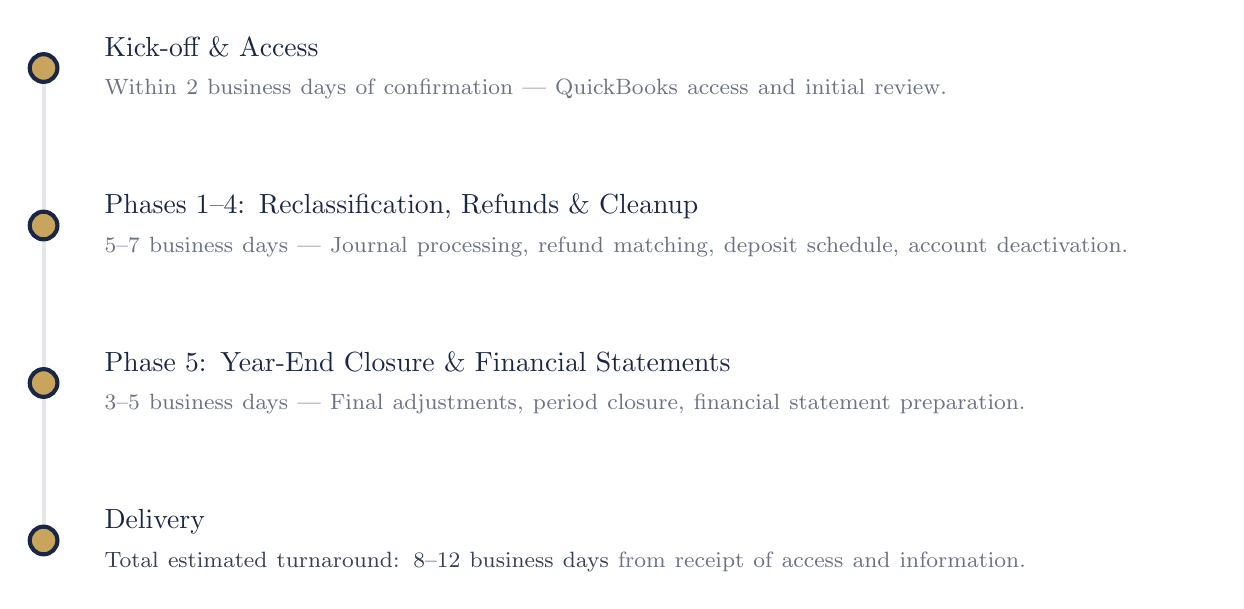
\begin{tikzpicture}
  % Timeline line
  \draw[grayline, line width=1.5pt] (0.35,-0.2) -- (0.35,-5.8);
  
  \fill[gold] (0.35,0) circle (5pt);
  \draw[navy, line width=1.5pt] (0.35,0) circle (5pt);
  \node[anchor=west, text width=140mm] at (1.0,0) {
    {\color{navy}\latosemibold\fontsize{10pt}{10pt}\selectfont Kick-off \& Access}\\[2pt]
    {\color{textmuted}\fontsize{8.5pt}{12pt}\selectfont Within 2 business days of confirmation --- QuickBooks access and initial review.}
  };
  
  \fill[gold] (0.35,-2.0) circle (5pt);
  \draw[navy, line width=1.5pt] (0.35,-2.0) circle (5pt);
  \node[anchor=west, text width=140mm] at (1.0,-2.0) {
    {\color{navy}\latosemibold\fontsize{10pt}{10pt}\selectfont Phases 1--4: Reclassification, Refunds \& Cleanup}\\[2pt]
    {\color{textmuted}\fontsize{8.5pt}{12pt}\selectfont 5--7 business days --- Journal processing, refund matching, deposit schedule, account deactivation.}
  };
  
  \fill[gold] (0.35,-4.0) circle (5pt);
  \draw[navy, line width=1.5pt] (0.35,-4.0) circle (5pt);
  \node[anchor=west, text width=140mm] at (1.0,-4.0) {
    {\color{navy}\latosemibold\fontsize{10pt}{10pt}\selectfont Phase 5: Year-End Closure \& Financial Statements}\\[2pt]
    {\color{textmuted}\fontsize{8.5pt}{12pt}\selectfont 3--5 business days --- Final adjustments, period closure, financial statement preparation.}
  };
  
  \fill[gold] (0.35,-6.0) circle (5pt);
  \draw[navy, line width=1.5pt] (0.35,-6.0) circle (5pt);
  \node[anchor=west, text width=140mm] at (1.0,-6.0) {
    {\color{navy}\latosemibold\fontsize{10pt}{10pt}\selectfont Delivery}\\[2pt]
    {\color{textbody}\latosemibold\fontsize{8.5pt}{12pt}\selectfont Total estimated turnaround: 8--12 business days} {\color{textmuted}\fontsize{8.5pt}{12pt}\selectfont from receipt of access and information.}
  };
\end{tikzpicture}

\pagefooter{5}

\clearpage

% ============================================================
% PAGE 6 — PRICING, REQUIREMENTS, TERMS
% ============================================================
\thispagestyle{empty}

\pageheader{6}

{\fontsize{15pt}{15pt}\selectfont\latosemibold\color{navy}\sectionnum{9}\;\;Your Investment}

\vspace{10pt}
\begin{tcolorbox}[colback=navy, colframe=navy, arc=6pt, boxrule=0pt, left=8mm, right=8mm, top=7mm, bottom=7mm]
{\color{gold}\latosemibold\fontsize{7.5pt}{7.5pt}\selectfont\addfontfeature{LetterSpace=8}ALL-INCLUSIVE FIXED FEE}\\[10pt]
{\color{white}\latoblack\fontsize{38pt}{38pt}\selectfont {\latolight\fontsize{16pt}{16pt}\selectfont\color{white!50}R\,}13,000}\\[5pt]
{\color{white!45}\latolight\fontsize{8.5pt}{8.5pt}\selectfont VAT Exclusive\;\textbullet\;No hidden hourly charges}\\[14pt]
{\color{white!80}\fontsize{9pt}{18pt}\selectfont
{\color{gold}\latosemibold\checkmark}\;\,Deposit reclassification (Revenue $\rightarrow$ Liability)\\
{\color{gold}\latosemibold\checkmark}\;\,Refund identification, allocation \& reconciliation\\
{\color{gold}\latosemibold\checkmark}\;\,Tenant deposit schedule preparation\\
{\color{gold}\latosemibold\checkmark}\;\,Account deactivation \& cleanup\\
{\color{gold}\latosemibold\checkmark}\;\,Financial year-end closure\\
{\color{gold}\latosemibold\checkmark}\;\,Financial statements (Income Statement, Balance Sheet \& Schedules)}
\end{tcolorbox}

\vspace{14pt}
{\fontsize{15pt}{15pt}\selectfont\latosemibold\color{navy}\sectionnum{10}\;\;What We Need From You}

\vspace{6pt}
\begin{itemize}[leftmargin=8mm, itemsep=4pt, label={\textcolor{gold}{$\circ$}}]
  \item {\color{textbody}\fontsize{10pt}{14pt}\selectfont QuickBooks access --- admin-level login or accountant invitation}
  \item {\color{textbody}\fontsize{10pt}{14pt}\selectfont Bank statements for the year (for reconciliation purposes, if required beyond bank feeds)}
  \item {\color{textbody}\fontsize{10pt}{14pt}\selectfont Notes on any tenant accounts to discuss before deactivation}
  \item {\color{textbody}\fontsize{10pt}{14pt}\selectfont Signed acceptance of this proposal to commence work}
\end{itemize}

\vspace{14pt}
{\fontsize{15pt}{15pt}\selectfont\latosemibold\color{navy}\sectionnum{11}\;\;Terms \& Conditions}

\vspace{10pt}
\begin{minipage}[t]{0.31\textwidth}
\begin{tcolorbox}[colback=graybg, colframe=graybg, boxrule=0pt, arc=3pt, left=3mm, right=3mm, top=3mm, bottom=3mm]
{\color{navy}\latosemibold\fontsize{9pt}{9pt}\selectfont Payment Terms}\\[3pt]
{\color{textmuted}\fontsize{8pt}{12pt}\selectfont 50\% deposit on acceptance. Balance of 50\% on delivery of financial statements.}
\end{tcolorbox}
\end{minipage}%
\hfill
\begin{minipage}[t]{0.31\textwidth}
\begin{tcolorbox}[colback=graybg, colframe=graybg, boxrule=0pt, arc=3pt, left=3mm, right=3mm, top=3mm, bottom=3mm]
{\color{navy}\latosemibold\fontsize{9pt}{9pt}\selectfont Validity}\\[3pt]
{\color{textmuted}\fontsize{8pt}{12pt}\selectfont This proposal is valid for \textbf{30 days} from date of issue (18 February 2026).}
\end{tcolorbox}
\end{minipage}%
\hfill
\begin{minipage}[t]{0.31\textwidth}
\begin{tcolorbox}[colback=graybg, colframe=graybg, boxrule=0pt, arc=3pt, left=3mm, right=3mm, top=3mm, bottom=3mm]
{\color{navy}\latosemibold\fontsize{9pt}{9pt}\selectfont Additional Scope}\\[3pt]
{\color{textmuted}\fontsize{8pt}{12pt}\selectfont Work outside this scope (e.g., prior-year corrections, SARS submissions) quoted separately.}
\end{tcolorbox}
\end{minipage}

\pagefooter{6}

\clearpage

% ============================================================
% PAGE 7 — ACCEPTANCE & SIGNATURES
% ============================================================
\thispagestyle{empty}

\pageheader{7}

{\fontsize{15pt}{15pt}\selectfont\latosemibold\color{navy}\sectionnum{12}\;\;Acceptance}

\vspace{8pt}
{\color{textbody}\fontsize{10.5pt}{16pt}\selectfont
To accept this proposal, please sign below or reply to the accompanying email confirming your agreement. Upon acceptance, we will issue an invoice for the 50\% deposit and schedule the kick-off within two business days.

We look forward to working with you and delivering a clean, compliant year-end for Property Denvour.}

\vspace{24pt}
\begin{minipage}[t]{0.46\textwidth}
\begin{tcolorbox}[colback=graybg!40, colframe=grayline, boxrule=0.5pt, arc=3pt, left=5mm, right=5mm, top=5mm, bottom=5mm]
{\color{navy}\latosemibold\fontsize{8.5pt}{8.5pt}\selectfont\addfontfeature{LetterSpace=4}CLIENT --- PROPERTY DENVOUR}\\[2pt]
\textcolor{gold}{\rule{\linewidth}{1.5pt}}

\vspace{30pt}
\textcolor{grayline}{\rule{\linewidth}{0.5pt}}\\[2pt]
{\color{textlight}\latolight\fontsize{7.5pt}{7.5pt}\selectfont Full Name}

\vspace{30pt}
\textcolor{grayline}{\rule{\linewidth}{0.5pt}}\\[2pt]
{\color{textlight}\latolight\fontsize{7.5pt}{7.5pt}\selectfont Signature}

\vspace{30pt}
\textcolor{grayline}{\rule{\linewidth}{0.5pt}}\\[2pt]
{\color{textlight}\latolight\fontsize{7.5pt}{7.5pt}\selectfont Date}
\end{tcolorbox}
\end{minipage}%
\hfill
\begin{minipage}[t]{0.46\textwidth}
\begin{tcolorbox}[colback=graybg!40, colframe=grayline, boxrule=0.5pt, arc=3pt, left=5mm, right=5mm, top=5mm, bottom=5mm]
{\color{navy}\latosemibold\fontsize{8.5pt}{8.5pt}\selectfont\addfontfeature{LetterSpace=4}SGBS GROUP PTY LTD}\\[2pt]
\textcolor{gold}{\rule{\linewidth}{1.5pt}}

\vspace{30pt}
\textcolor{grayline}{\rule{\linewidth}{0.5pt}}\\[2pt]
{\color{textlight}\latolight\fontsize{7.5pt}{7.5pt}\selectfont Sibusiso Mavuso}

\vspace{30pt}
\textcolor{grayline}{\rule{\linewidth}{0.5pt}}\\[2pt]
{\color{textlight}\latolight\fontsize{7.5pt}{7.5pt}\selectfont Signature}

\vspace{30pt}
\textcolor{grayline}{\rule{\linewidth}{0.5pt}}\\[2pt]
{\color{textlight}\latolight\fontsize{7.5pt}{7.5pt}\selectfont 18 February 2026}
\end{tcolorbox}
\end{minipage}

\vspace{40pt}
\begin{center}
\textcolor{grayline}{\rule{0.8\textwidth}{0.4pt}}\\[8pt]
{\color{textlight}\latolight\fontsize{7pt}{7pt}\selectfont\addfontfeature{LetterSpace=6}CONFIDENTIAL\;\textbullet\;SGBS GROUP PTY LTD\;\textbullet\;INSPIRING DREAMS}
\end{center}

\pagefooter{7}

\end{document}
